\chapter{系统设计与实现}

\section{系统设计目标与需求分析}

本自动驾驶系统希望能够打造一个有物理精准性、算法高效性以及强可验证性的虚实交互闭环体系,依靠融合数字孪生技术与强化学习框架,让虚拟小车在仿真环境里达成自动驾驶,为此系统要拥有以下核心功能:能在用户给出的仿真环境中开展自动驾驶模型训练,使用户可借助调整奖励函数的各类参数来调适模型,让训练得出的模型契合用户需求。本系统的主要以便搭建一个可训练、可测试且可交互的自动驾驶平台,要可在复杂动态环境中提供快速、精确且安全的自动驾驶服务,这也是当今自动驾驶技术发展的一项关键技术,它可细分为功能需求和非功能需求。

\subsection{功能需求}

根据系统功能需求的分析情况,本研究要达成以下几个核心模块,其一要开发出有较高真实度的车辆运动控制系统,该系统包含转向引导以及速度调控功能,其二要搭建强化学习训练平台,以此来支撑智能体在路径规划以及动态避障任务方面的学习进程,其三要整合激光雷达与碰撞检测传感器系统,实现对动态障碍物的实时感知以及反馈机制。其四要设计可视化交互界面,用于系统参数配置以及训练过程的可视化监控。

\subsection{非功能需求}

系统应当支持在Windows系统之上运用Carla仿真平台来运行,同时还要有较高的鲁棒性以及较低的资源消耗情况,并且用户可依据自身意愿自由地选择其所希望使用的强化学习算法模型,强化学习训练过程要保持稳定,而且有一定的扩展能力,用户交互界面需要拥有较强的人机交互性能,并且操作简洁。


\section{开发环境}

本研究是于windows11操作系统环境下,借助Pycharm开发平台,以TensorFlow深度学习框架为基础,运用Python编程语言展开开发工作,并在完成对训练好的模型进行封装后得以实现,针对基于数字孪生的自动驾驶强化学习仿真系统的操作界面,运用PyQt5进行了简易制作,以此达成对Carla仿真环境中小车的自动驾驶操作。

\begin{table}[htbp]
	\centering
	\caption{开发环境配置}
	\label{tab:actuators}
	\begin{tabular}{lll}
		\toprule
		\textbf{开发平台} & \textbf{软件环境} & \textbf{硬件环境} \\
		\midrule
		PC   &操作系统:Windows 11   &  CPU:Intel(R) Core(TM) i7-12700H  \\
		PC &开发语言:Python       & GPU:NVIDIA GeForce RTX 3060 \\
		PC &IDE:PyCharm          &  \\
		\bottomrule
	\end{tabular}
\end{table}

\section{系统总体设计}
\subsection{设计概要}
如图3-1所示为本篇文章的系统设计架构,文章中的系统能在用户界面帮助使用者选择Carla仿真地图来运行自动驾驶模型、选择算法及算法模型,并且可进行训练或测试,当用户训练所选算法模型时,还可调整训练参数,以使训练出的模型更契合使用者的具体需求。

\begin{figure}[hbt]
	\centering
	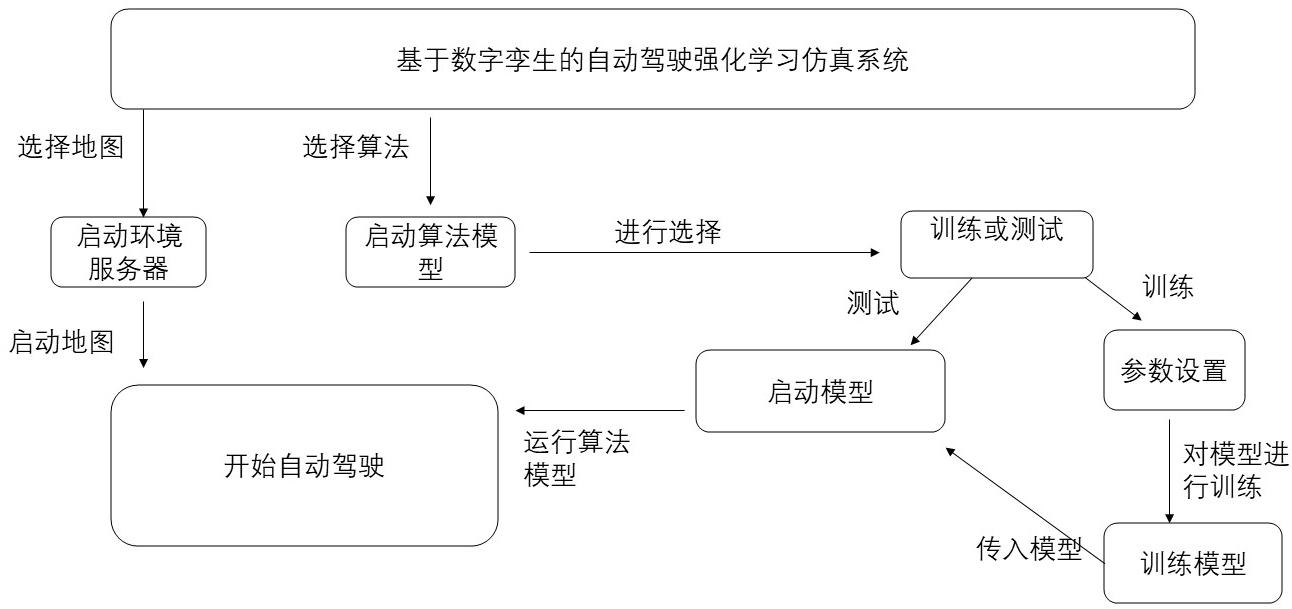
\includegraphics[width=\linewidth]{系统设计架构图.jpeg}
	\caption{系统设计架构图}
	\label{f.example}
\end{figure}

本系统运用三层结构展开设计,按照从下往上的次序依次为底层感知层、中间控制逻辑层以及用户交互层,底层感知层承担着连接Carla仿真平台的任务,同时负责控制环境生成、地图加载以及传感器初始化,借助Python API达成车辆生成、目标点设定以及路径规划点采样,并且附加激光雷达和碰撞传感器用以进行实时环境感知。中间控制逻辑层作为系统核心逻辑处理部分,覆盖强化学习环境定义、奖励函数体系、PPO训练框架等内容,在训练阶段,环境依据动作返回奖励并更新状态,于推理阶段,策略网络针对当前状态做出行动决策,用户交互层基于PyQt5构建GUI,用户可可视化设置参数,并实时查看导航状态、训练进度、路径规划图等情况。

\subsection{用户交互模块}
本系统围绕PyQt5展开设计与构建工作,借助Qt框架里的QImageReader类达成对多源传感器数据的兼容性支持,像摄像头RGB图像、激光雷达点云以及车辆状态数据等都囊括在内,面对动态仿真场景的需求,该系统可实时解析数字孪生环境所产生的时序数据流,并且借助首帧快照预览功能帮助用户迅速定位关键训练片段。在数据预处理阶段运用EXIF元数据校验与坐标系归一化技术,以此保证多模态数据在时空维度上实现对齐,给强化学习模型提供一致性输入。

此系统运用Model-View-Controller架构达成高内聚低耦合设计,当中的模型层借助集成数字孪生环境引擎、强化学习算法以及多传感器融合模块,达成实时仿真推演、策略优化以及数据特征提取,视图层则凭借提供三维可视化视窗、训练指标仪表盘以及控制面板,支持用户以多视角观察车辆行为。系统里的控制层借助信号-槽机制协调用户交互事件,如场景加载、训练启停、参数调整等,依靠协调这些用户交互事件保证界面响应与仿真计算的异步协同。

为了实现跨设备的兼容性,系统采用了响应式界面适配策略,该策略首先设定了基础尺寸约束条件,将最小窗口尺寸规定为1280×720像素,以保证在最小视口情况下内容仍能完整呈现,保障系统的基本可用性,在此基础上,系统引入了动态布局调整机制,依靠将控件的sizePolicy属性设置为Expanding,建立起窗口尺寸与控件大小的联动关系,实现控件按比例缩放,保证界面布局在不同尺寸的设备上可保持良好的视觉效果和可用性。

在核心交互组件的实现进程里,数字孪生视图是依据Qt框架的QOpenGLWidget来构建的,深度融合了Carla/SUMO仿真引擎,可支持高精度车辆动力学模型以及天气系统的实时渲染,其中天气系统涉及雨雾模拟、昼夜光照变化等内容,又借助setScissorTest技术来优化视口裁剪,使得复杂城市场景的渲染效率得到了提升。训练监控模块运用QCustomPlot定制开发了多维训练曲线仪表盘,它可动态呈现累计奖励、Q值波动等关键指标,支持拖拽缩放交互以及数据点悬停详情展示,并且利用标注功能对策略收敛阶段、探索-利用转换节点等关键训练事件进行可视化标记,为算法调优提供直观依据。在参数管理方面,凭借QTreeWidget实现了树形结构化超参数编辑器,对深度强化学习算法参数、环境物理特性配置以及传感器噪声模型进行分层组织,内置参数范围校验机制和预设方案快速加载功能,以此保证实验参数有可控性与可复现性,系统还配备了基于QTextBrowser的实时日志组件,采用多级色彩编码来区分信息、警告和错误事件,集成正则表达式过滤功能,支持对紧急制动、路线偏离等关键操作的时序回溯分析,形成完整的训练过程审计链条。


本系统的控制子系统依靠Qt的信号—槽机制来达成业务逻辑,保证用户操作流程得以顺畅,界面也可维持稳定,其具体设计内容如下:用户首先于控制面板挑选强化学习算法,以此确定采用何种强化学习算法模型来展开训练或测试,接着选择具体的训练模型来对其开展测试或训练,随后选择运行的Carla仿真地图,让自动驾驶小车在其上进行显示。最后选择对算法模型进行训练或测试来实际运行模型。图3-2为用户操作流程图,其清晰地描述了用户与系统之间的交互逻辑。

\begin{figure}[hbt]
	\centering
	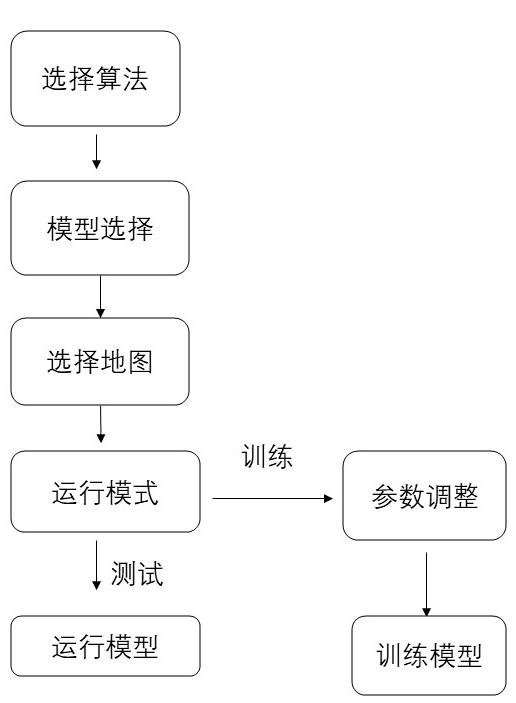
\includegraphics[width=0.4\linewidth]{用户操作流程.jpeg}
	\caption{用户操作流程}
	\label{f.example}
\end{figure}

该系统的核心优势呈现于多维度的技术创新以及用户体验优化方面,借助多模态融合可视化技术把抽象的强化学习过程和具象化的三维驾驶场景深度融合,在实时渲染的车辆轨迹、障碍物交互里直观呈现策略决策逻辑,提高了算法透明度与策略可解释性,构建交互式参数调节体系,可凭借可视化控件直接动态调节深度强化学习超参数,并同步观测训练指标和驾驶行为的实时变化,缩短了算法调优周期,系统运用响应式布局架构与自适应的渲染策略,达成从高性能桌面工作站到移动终端的无缝体验转移,保证不同硬件环境下界面功能与视觉呈现的一致性,在实时性上,依靠异步计算架构与GPU并行加速技术,即便在4K高分辨率情况下仍可维持每秒30帧以上的流畅仿真交互,保障大规模城市场景中传感器数据流、物理引擎与策略推理的高效协同,为复杂自动驾驶任务的强化学习训练提供毫秒级响应的沉浸式数字孪生环境。

\subsection{功能展示模块}
在本篇文章里,系统的功能展示模块借助数字孪生所提供的虚实交融交互设计以及多维数据协同,打造出了覆盖算法训练、场景验证以及策略优化的全流程技术闭环,此模块以沉浸式数字孪生环境为基础,深度融合物理仿真引擎与强化学习框架,实现了三大核心功能体系的有机联动。

该系统利用Carla仿真为虚拟小车提供训练和测试所需的仿真环境。系统集成了Carla的引擎架构,支持毫米波雷达点云、摄像头RGB图像、IMU惯性数据等多模态传感器仿真,并且允许动态调整传感器噪声模型,比如高斯噪声强度、运动模糊参数等,可精准复现边缘案例下的感知退化场景,借助拖拽式障碍物生成工具,用户可以在三维视图中实时添加突发行人穿行、车辆违规变道等高风险事件,构建渐进式课程学习环境。

该系统的强化学习训练中枢功能打造了端到端的策略优化途径,能支持像PPO、SAC、DQN等主流算法实现即插即用式的部署,训练界面设有策略蒸馏可视化面板,可实时呈现价值函数热以此来、动作选择概率分布以及探索轨迹熵值的变化情况,利用颜色梯度映射来揭示策略网络在状态空间里的决策偏好。用户可以借助交互式超参数面板动态调节折扣因子、经验回放权重等核心参数,还可以借助对比实验管理功能并行运行多组参数配置,系统会自动生成训练曲线对比矩阵以及收敛效率分析报告,加快算法调优的进程。

而该系统的实时诊断与干预功能构建了双向可控的仿真生态,在自动驾驶策略执行时,系统会借助多维仪表盘同步显示车辆动力学状态、环境交互指标以及奖励函数构成。当检测到策略失效风险时,用户能借助“人工接管”模式直接注入控制指令,系统会自动记录干预前后的状态转移差异,并且触发策略漏洞分析模块生成修复建议,所有训练过程都支持全程录制以及关键帧标记,用户可以凭借时空滑动条回溯任意时刻的多传感器数据流,结合策略决策热以此来进行根因分析,形成“训练-验证-修正”的强化学习提高回路。

\subsection{结果展示模块}

数字孪生的自动驾驶强化学习仿真系统里有个结果展示模块,依靠多维度的数据呈现加上深度分析,搭建起从实时决策到策略优化的完整反馈闭环,这个模块有基础状态反馈、动态可视化推演以及结构化策略评估这三个核心功能,能全方位解析自动驾驶模型在虚拟环境中的行为逻辑与学习效能。

基础状态反馈模块会实时输出车辆核心运行指标,像是当前决策动作,包含转向角度、加速度、制动强度,以及环境交互状态,有碰撞概率、车道偏离距离,以及策略置信度,是以百分比形式动态显示的,其中决策动作借助阈值判定机制被分类成“安全操作”或者“风险行为”,并且采用红绿双色编码来进行视觉警示,置信度进度条会同步映射模型对当前动作的确定性评估,以此帮助用户快速捕捉关键决策节点。

动态可视化推演模块将数字孪生环境和强化学习过程进行深度融合,利用三维渲染引擎实时呈现车辆轨迹预测、障碍物交互热以此来以及价值函数空间分布,热以此来生成运用多尺度注意力机制,结合时空特征金字塔网络提取道路场景的语义权重,在经双线性插值还原至原始点云分辨率后,采用光谱映射技术直观标注模型决策焦点。同步叠加的Q值云图借助半透明色域层呈现状态空间的策略价值分布,动态揭示强化学习策略的探索与利用平衡过程,

结构化策略评估报告以多维度指标体系作为核心,覆盖训练阶段诊断、场景适应性分析以及安全审计日志,报告整合DRL超参数配置与环境动力学参数,依靠关联性分析生成优化建议,例如针对连续弯道场景的转向响应延迟问题,系统会自动推荐调整策略网络的梯度裁剪阈值或者增加课程学习难度梯度。所有分析结果支持导出为标准化技术文档,包括可交互的时序数据图表与场景回放链接,为算法迭代提供可追溯的基准参照。

\section{系统编码与实现}
\subsection{环境模块实现}


借助Carla仿真模拟可构建出虚拟仿真环境,Carla仿真平台可用于测试针对复杂规划任务的决策算法性能,在算法训练进程以及基于车辆生产状况展开研究时可发觉,要是在真实道路上开展自动驾驶测试,车祸发生概率颇高,会致使道路基础设施遭受损害以及造成重大物质损失。在实际研究里,要高度逼真地模拟重型机械的显示画面,把从各类实验收集的数据当作输入数据添加进去,还将真实路况的相关信息输入到仿真平台中,以此构建仿真环境,增添油门、转向和刹车等车辆相关数据,达成整体仿真。

我们可借助Carla模拟器开展自动驾驶系统的测试工作,Carla模拟器有支持各类复杂交通场景的能力,如此一来,科学家可运用可视化工具动态调整输入与输出参数,还可把来自多模态传感器如激光雷达点云、摄像头图像以及毫米波雷达信号等的数据导入系统,以此达成高效的数据集成以及闭环验证。就以CARLA模拟器来说,该平台是基于虚幻引擎4搭建而成的,并且运用基于物理的渲染技术PBR达成逼真的光影效果,其动态天气系统模拟出了雨、雪、雾等恶劣天气状况,它按照时区控制的昼夜循环运行,为测试算法提供了多维环境,核心引擎是用C++编写的,且与Python API兼容,这让开发人员可以最少的代码实现深度定制,同时能快速调用更高级别的接口来获取车辆状态、道路拓扑以及位置数据。

经研究发现,CARLA\cite{dosovitskiy2017carla}模拟器运用OpenDrive标准剖析真实道路的几何参数与交通规则,还可以把高分辨率地图数据转化成可编程的虚拟场景,其模块化架构让研究人员可详细描述车辆动力学模型,像轮胎摩擦系数、传动效率等,以及传感器噪声特性,例如雷达检测误差模型,以及道路使用者行为,比如行人接近概率等的独立性。在复杂军事设施建设方面,Carla仿真平台的军事设施细节库能用来创建特殊区域,像指挥中心和装甲救护车停车场,依靠结合可定制的通信干扰模型以及电磁环境参数,可有效模拟战场上自动驾驶任务的需求,CARLA分布式计算系统支持多智能体协同仿真,借助ROS桥接接口可轻松连接到机器人操作系统。这为多车辆编队规划和V2X通信等复杂任务提供了认证路径。

Carla模拟器能为感知系统训练带来诸多优势,其仿真平台的物理引擎可精准模拟光传播路径,为计算机视觉系统提供符合真实光学定律的图像信息,借助API操作Carla能实时访问传感器元数据,像摄像头内外参数、雷达采样率等,推动多传感器融合算法开发,Carla仿真平台还支持用GPU加速生成大规模点云,契合激光雷达感知算法对数据处理效率的需求。CARLA开源社区生态系统持续发展,催生出丰富插件库,囊括强化学习接口、交通流生成工具和异常事件触发器等模块,这让研究人员能直接调用自定义函数,也能用C++/Python混合框架扩展自定义函数,借助这套高度开放且技术先进的仿真系统,从基础环境原型设计到复杂系统验证的整个研发流程可在单一平台完成。这减少了自动驾驶技术从实验室到实际应用的工作量。

经观察可知,CARLA模拟器相较传统模拟平台呈现出十分突出的技术优势,它运用模块化架构以及强大的开放生态系统,为自动驾驶系统开发创设了极为灵活的实验环境,Carla仿真平台以虚幻引擎4搭建而成,有游戏级物理渲染能力,借助混合C++/Python编程接口,达成了底层代码优化与高层视觉操作的良好结合。其多客户端架构支持分布式计算,可在单个计算节点上并行开展多个模拟过程,此设计颇为契合多智能体协作、车路云融合等复杂场景下的验证需求。

在功能扩展性上,CARLA 提供了 20 多种 API 库,涉及环境感知、运动控制、交互等核心内容,开发者能借助车辆物理 API 微调车辆动力学参数,如传动效率与轮胎摩擦系数,还可以利用 World API 动态改变道路拓扑,像添加施工时区,开发人员也可运用 TrafficManager API 编程交通流模式,细致管理人行道、车道变换逻辑以及交通信号灯相位。环境建模系统值得关注,它支持 16 种预定义天气类型,包含大雨、大雪、浓雾等极端条件,能将光强度精确调整到勒克斯级别,集成基于物理的材质渲染 (PBR) 模型,保证摄像机收集的场景数据与真实光学特性相符。

可发现Carla的空间分辨率削减了传统地理边界,对现有的OpenDrive网络给予支持,还让研究人员可调整地图大小以达成最大程度的可重复性,Carla仿真平台有丰富的建筑材料库,可迅速建造军事基地以及如兵营、营房、补给基地等特定地点,除激光雷达、摄像头和毫米波雷达外,CARLA还设有噪声检测和存储系统。比如凭借改变激光雷达视场或者GPS导航模式,就能测试算法的可靠性。

在使用Carla仿真平台之际,需留意CARLA开源社区当前处于功能演进进程,此库有先进自学习能力、5G通信支持、独特生成器等多项特性,研究人员能借助ROS桥与机器人流程交互,又能凭借Python脚本快速生成自定义消息,Carla仿真平台为自动驾驶汽车控制算法奠定坚实基础,也为智能车辆控制、战场模拟、车辆导航及训练等应用开拓诸多可能。针对图3-3所示应用,CARLA在车辆停车识别、紧急数据检索、个人数据管理等复杂任务中表现出优异性能。

\begin{figure}[hbt]
	\centering
	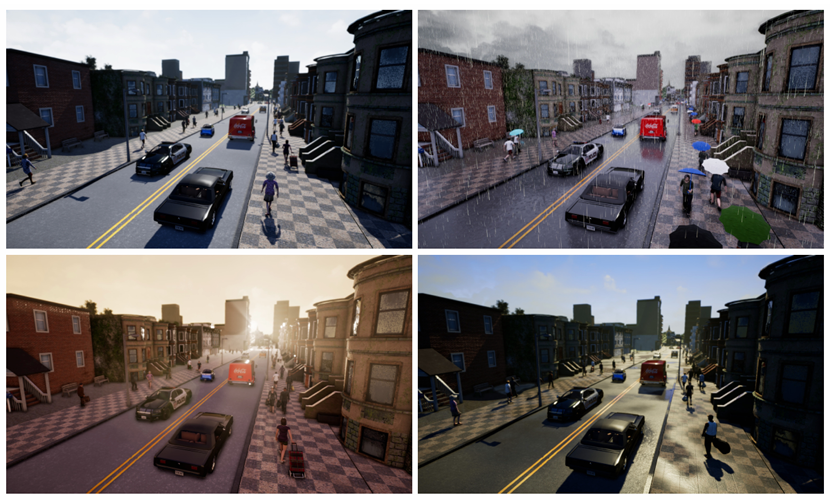
\includegraphics[width=\linewidth]{仿真环境中的不同天气.png}
	\caption{仿真环境中的不同天气}
	\label{f.example}
\end{figure}

借助研究可发现,Carla模块化的传感器接口系统,使得CARLA模拟器可较为轻松地与多种类型传感器实现集成,像LiDAR、全球定位系统也就是GPS、测量单元即MU以及RGB摄像头等,当用户认真阅读传感器配置指南之后,借助GUI或者Python脚本,可快速对多个传感器参数加以配置,覆盖激光雷达扫描速率比如10/20 Hz、GPS位置噪声模型其可模拟真实信号的波动特性、摄像机分辨率支持720p到4K的范围以及安装位置由坐标系转换工具精确确定。专门针对该平台设计了传感器冗余机制,要是用户没有主动配置特定传感器,系统会自动让内置的虚拟传感器填补数据空白,比如软件生成的惯性测量单元即IMU数据用来提供车辆运行状况信息并维护模拟实验的完整性。

我们通过研究发现,在Carla传感器放置方面,CARLA 支持多摄像头共配置模式,并允许研究人员在单个模拟步骤中创建多维观察系统。例如,智能汽车可以同时部署远距离前置摄像头(模仿特斯拉的三摄像头Autopilot架构)、广角后置摄像头(用于停车检测)以及两侧鱼眼镜头(用于覆盖交叉路口的盲点)。我们为了满足特定的任务需求,可以通过API动态添加红外热成像、毫米波雷达等专用传感器,并通过ROS消息总线或CarlaPy API将其数据流实时发送到算法处理模块。这种灵活的配置能力使研究人员能够准确模拟真实车辆中的传感器阵列,并提供接近真实车辆的测试条件以开发多模式数据融合算法。

该平台提供的传感信息远远超过传统成像设备所使用的传感信息。除了传统的 RGB 图像和点云数据外,它还符合 ASAM 标准,包括逻辑分割图像(每个像素标记为道路、行人、汽车等)、模式分割掩码(用于识别不同的目标类型)和动态物体轨迹预测数据(包括未来 5 秒内运动的概率分布)。对于图3-4所示的典型传感器数据,系统可以使用原始传感器数据、预处理的框检测信息(带有准确度分数)和高清匹配结果来构建从原始观测到数据集的整个数据链。这种传感数据层次的细粒度结构始于基本特征提取。它为深度学习算法提供了广泛的训练对象,包括复杂的场景识别。

为了追踪道路使用者的姿势,CARLA 将物理引擎与 AI 行为模型相结合,以获得车速(精确到 0.1 公里/小时)、加速度(包括纵向和后向偏航角)和偏航角(精确到0.1度)等关键参数的实时估计。可显示碰撞警告标志、违规标志(如闯红灯、非法变道等)。这些丰富的数据为开发强化学习算法的成本函数提供了定量基础。特别是在多智能体协作场景中,采用分布式传感器数据的时间同步方法(误差小于5毫秒)可以准确地重建车辆之间的通信游戏计划,为学习团队的智能决策算法创建数据库。

\begin{figure}[hbt]
	\centering
	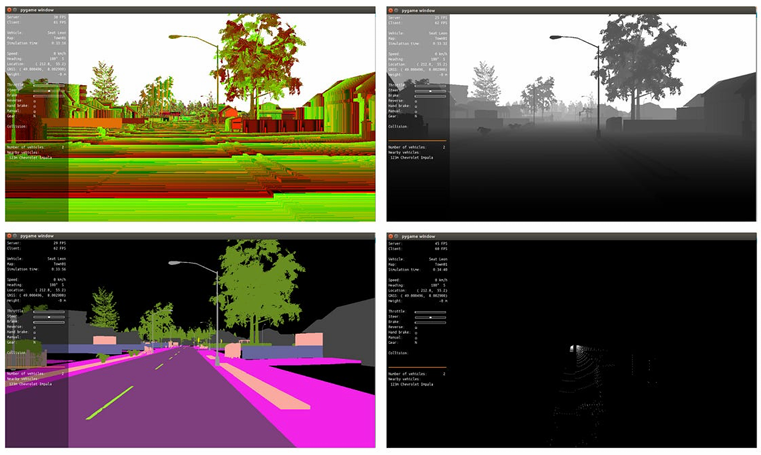
\includegraphics[width=\linewidth]{CARLA环境数据.png}
	\caption{CARLA环境数据}
	\label{f.example}
\end{figure}

本研究为仿真实验开发的CARLA平台控制系统如表3-2所示。在操作系统的选择上,考虑到Windows系统在工程开发领域的广泛应用(例如,兼容重要的IDE工具链、支持DirectX图形界面以及应对破坏性环境的特殊情况),研究团队决定使用该环境作为主要开发的基础。在实施过程中,定义了一套预处理的环境元素(包括精确地图、交通信号灯数据和3D模型库)以及一个可定制的道路网络模型(基于OpenDrive平台构建,包含直线、曲线、弯道等常用组件)。CARLA官方发布的跨平台程序(基于CMake构建系统)和Visual Studio 2019环境,编译了基础代码以创建一个完整的框架,其中包括核心仿真引擎和用于该环境的Python API库。

\begin{table}[htbp]
	\centering
	\caption{软硬件配置信息}
	\label{tab:config}
	\begin{tabular}{ll}
		\toprule
		\textbf{名称}         & \textbf{型号版本}               \\
		\midrule
		操作系统            & Windows 11                     \\
		CPU               & Intel(R) Core(TM) i7-12700H    \\
		GPU               & NVIDIA RTX 3060 (6GB)          \\
		Python            & 3.7.0                          \\
		TensorFlow        & 2.11.0                         \\
		Carla             & 0.9.14                         \\
		TF-Agents         & 0.3.0                          \\
		Pygame            & 1.9.6                          \\
		Gym               & 0.12.5                         \\
		Torch             & 1.13.1                         \\
		\bottomrule
	\end{tabular}
\end{table}


该架构平台具有独特的功能:一方面,通过开放的交互层(例如Vehicle API和World API),可以调用200多个函数来实现车辆动态的变化(例如齿轮比调整),并为动态传感器系统输入光照和时间信息(例如);另一方面,利用虚幻引擎4的对象和绘图搜索系统,可以创建军事禁区、气象试验场等特殊场景。主程序CARLA.exe采用分布式多客户端架构设计,并可通过TCP/IP协议在节点之间进行同步,这为进一步开发多智能体控制算法提供了基础。

\subsection{奖励函数实现}

我们通过研究发现,奖励函数是强化学习过程中的关键环节,直接影响智能体的行为。设计合理的奖励函数可以显著提升学习效率。当奖励函数准确及时地反映有益行为时,可以加快智能体的学习进程,并帮助其更快地达到预期的性能水平。考虑到自动驾驶任务中的奖励函数,如果存在真实的奖励函数,则该函数很可能是多状态的,因为人类驾驶员会根据情况改变目标。为了简化问题,下文用于自主控制任务的深度强化学习模型通常将奖励函数表示为因子的线性组合,观测参数在当前时刻很容易获得为标量,从而易于求解。大多数关于驾驶安全性和高速驾驶效率的研究都考虑了实际车辆方向和道路方向的稳定性。

我们需要根据上述原则来考虑车道保持任务场景,确定通用奖励函数$𝑅_1$以防止车道偏离和碰撞,如公式3.1所示。该公式使得智能汽车能够学习沿着车道中心线行驶,或按照专家指示的路径点行驶至目的地。该方法直观地体现了汽车与道路对齐的重要性,并在汽车正确对齐时提供积极的反馈,从而促进稳定安全的驾驶。

\begin{equation}
	R_1 = v_x \cos(\theta_l) - v_x \sin(\theta_l) - v_x \lvert d \rvert - C
\end{equation}

奖励函数$𝑅_1$可以引导代理沿着轨道轴快速行驶,重点是提高速度并在高速下保持稳定性。如果$𝜃_𝑙$过大,即车辆方向偏离了中心线,$𝑣_𝑥 cos(𝜃_𝑙)$的值将减小,$𝑣_𝑥 sin(𝜃_𝑙)$的值将增大。我们也可以从上述公式知晓整个公式的值可能变为负数。我们为了避免这种情况,可以鼓励车辆提高纵向速度,以减少车辆横向速度造成的功率损失。同时,术语$𝑣_𝑥|𝑑|$这也会惩罚与路缘的距离,减少车辆离路缘太近的可能性,从而避免转弯时转向困难的问题。$𝐶$是一个常数项,它允许将奖励函数设置为超参数,以便针对不同的车型、不同的环境或不同的驾驶轨迹进行优化。我们通过研究发现,经验丰富的驾驶员通常会在直路上尽可能加速,并在接近弯道时减速以确保平稳行驶。为了更好地匹配人们的驾驶习惯。因此,引入曲线感知距离$𝜎$作为状态空间中观测值的函数$𝑅_2$根据\cite{zou2021deep}的思想定义如下:

\begin{equation}
	\begin{split}
		R_2 &= \left( v_x \times \left( \frac{1 - \kappa_v \times \lvert v_x - v_a \rvert}{\beta} \right)^{\eta_1} \right) \\
		&\quad \times \left[ \cos \theta_l \times (1 - \lvert \sin \theta_l \rvert) \times (1 - \lvert d \rvert) \right] \\
		&\quad \times \left( \frac{\lvert \sigma \rvert}{50} \right)^{\eta_2},
	\end{split}
\end{equation}

其中$𝛽,𝜂_1,𝜂_2,𝜅_𝑣$是奖励的超参数,$𝑣_𝛼$表示弯道中的目标车辆速度,$𝛽,𝜅_𝑣$是用于规范速度差异的缩放因子,确保奖励在一定范围内。$𝜂_1$和$𝜂_2$为切换方案,将其值修改为{0,1},以限制速度。根据公式(3.2),连接根据曲线的距离$𝜎$发生。

\begin{equation}
	\eta_1, \eta_2 = 
	\begin{cases} 
		(1, 1) & \text{if } \sigma \leq 10, \\ 
		(0, 1) & \text{if } 10 < \sigma \leq 50, \\ 
		(0, 0) & \text{if } \sigma > 50. 
	\end{cases}
\end{equation}

理论上,$𝜎 ≤ 10$表示曲线正在接近或已经在曲线内部。此时,设置$𝜂_1 = 𝜂_2 = 1$得到奖励函数 (3.3)。在这种情况下,如果智能车辆的速度与目标速度偏差$𝑣_𝛼$,就会受到更严厉的惩罚。

\begin{equation}
	R_2 = v_x \times \left( \frac{1 - \kappa_v \times \lvert v_x - v_a \rvert}{\beta} \right) \times \left[ \cos \theta_l \times (1 - \lvert \sin \theta_l \rvert) \times (1 - \lvert d \rvert) \right] \times \left( \frac{\lvert \sigma \rvert}{50} \right)
\end{equation}

当$10 < 𝜎 ≤ 50$; 表示车辆将进入弯道。此时$𝜂_1 = 0$和$𝜂_2 = 1$,奖励函数变为(3.4)。
$𝜂_2$鼓励汽车微调方向,准备驶入弯道。

\begin{equation}
	R_2 = v_x \times \left[ \cos \theta_l \times (1 - |\sin \theta_l|) \times (1 - |d|) \right] \times \left( \frac{|\sigma|}{50} \right)
\end{equation}

当$𝜎>50$时,这意味着汽车在直线上行驶,前方没有弯道,因此$𝜂_1=𝜂_2=0$,奖励函数变为(3.5)。

\begin{equation}
	R_2 = v_x \times \left[ \cos \theta_l \times (1 - |\sin \theta_l|) \times (1 - |d|) \right].
\end{equation}

我们知道在自动驾驶中,安全至关重要,避免事故至关重要。根据 Levinson 等人的研究\cite{levinson2011towards}。我们可以知道,一个好的防撞策略必须仔细考虑车辆的特性、环境的不确定性以及其他车辆和行人的行为。按照这个想法,汽车的自动驾驶模型应该严厉惩罚汽车在碰撞过程中的行为,智能控制器应该学会在看到静态和动态问题时立即停车。记录碰撞预防逻辑来确定列表中的每个控制周期内是否发生碰撞。这些条目根据模拟器本身发生的碰撞检测返回“True”或“False”。当在历史列表中检测到碰撞时,立即使用关键惩罚。智能车会在反复碰撞中通过反复试错逐渐避免碰撞,因此惩罚量应该尽可能大,如公式(4.8)所示。

\begin{equation}
	R_{\text{reward\_collision}} = 
	\begin{cases} 
		-100, & \text{如果检测到碰撞}, \\ 
		0.5,  & \text{无碰撞}. 
	\end{cases}
\end{equation}

我们通过研究发现,通过对碰撞的严厉惩罚,能够有效地促使自动驾驶系统采取措施避免碰撞,增强整体的行车安全。自动驾驶的另一个关键方面是执行交通规则和法规。这些规则的执行首先将确保交通效率并防止不必要的拥堵和混乱。其次,交通规则的执行增加了车辆行为的可预测性。其他驾驶员和行人可以预测遵守规则的车辆的行为,从而降低潜在碰撞的可能性,并有助于学习方程(3.7)中的避碰策略。由于所提出的模型是基于城市交通状况的,车辆在经过路口时无法转入直车道。如果你转弯,对面驶来的车辆将被罚款。让我们定义奖励规则,$𝑅$规则,如公式 (3.8) 所示。这种设计确保代理遵守交通规则并避免在错误的车道上行驶。避免在错误的车道上行驶时频繁闯红灯。

\begin{equation}
	R_{\text{rules}} = 
	\begin{cases} 
		-10, & \text{如果不在正确的车道或逆行或闯红灯}, \\ 
		5,   & \text{正常情况}. 
	\end{cases}
\end{equation}

当我们于Carla仿真内安装数字模型之后,模拟器里触发的事件会被用来验证车辆是否契合规则,Carla仿真所模拟的世界里有着全部的电磁物质,而且这些电子之间会产生相互作用,每一个激光器的影响范围被设定成10米,要是和车辆的距离小于这个数值,那么交通信号灯状态就会恢复,同时会对车辆作出闯红灯的处罚。在路径分析过程中,最大路径数被设定为$l_m$,每一条路径$l_i$都有唯一的标识符,正数意味着车道处于车辆右侧,负数则意味着车道处于车辆左侧,要是发现了错误的联赛,便可产生奖励。

研究发现舒适性属于一种补偿设计方法,可鼓励平稳加速与减速,以此提高驾驶体验,这可抑制突然加速或者减速,达成对汽车的平稳控制,本文设计逻辑依据车辆加速度与转向角这两个物理量,研究发现突然变化会使乘客感觉不舒服,大的变化或许会致使车辆偏离道路,舒适性可车辆在加速度快速或突然变化以及转向角大幅变化时保持平稳行驶状态。这里运用二次公式,具体如下:

\begin{equation}
	R_{\text{comfort}} = -0.25 a_c^2 - \kappa_s \times \Delta \text{steer}^2
\end{equation}

基于特定研究方向,在自主控制模型训练进程里,模拟器运用动态图像更新方式构建虚拟控制环境,每当系统算出给定解决方案的成本值,环境模块便会自动把包含纵向加速度与横向加速度分量的加速度数据以及当前时刻的前轮转向角值存入历史数据库,创建实时序列,这种基于时间窗口的先进更新策略能让客户持续检测车辆运动特性,为后续决策提供完备运动学背景。

从动态驾驶这一角度而言,维持加速度与转向角之间的平稳过渡对达成安全舒适的驾驶体验意义重大,就长期控制来讲,运用PID控制算法来调控扭矩,把加速度变化率即误差值限定在±0.3m/s3以内,可有效避免突然加速或因冲击导致的倒塌情况,比如若当前车速与目标车速存在差距,控制系统会采取低速控制策略,而非直接施加制动力与转向力。在横向控制方面,基于模型预测控制也就是MPC的转向决策系统会将前轮转向速度限制在±15°/s,同时优化后续500毫秒的转向路径,这能保证正确的转向响应时间,又能防止因方向盘振动致使车辆转向角度出现突然变化。

经研究发觉,平稳控制策略有几个方面优点,其一借由最大程度减少各个方向加速度的陡然变化,车辆俯仰角可被控制在3°以内,可降低快速变化方向时翻车风险,其二持续行驶能保证轮胎滑移角维持在线性工作范围之内,防止因过度行驶致使轮胎受力过大而出现强度损失风险,其三高效加减速可使撞击速度增幅降低72\%,这对配备死亡监测系统的车辆颇为关键,若标准横向加速度测量控制在0.08g以下,90\%的乘客不会受伤。从学习系统角度而言,有效建模物理约束可让强化学习代理在探索策略空间时避开不良做法,其统一政策于国际道路测试中始终保持着98.7\%的成功率。

综合考虑上述式子,定义总体奖励函数$𝑅_{total}$:

\begin{equation}
	R_{\text{total}} = R_1 + R_2 + R_{\text{reward\_collision}} + R_{\text{rules}} + R_{\text{efficiency}} + R_{\text{comfort}}
\end{equation}

研究发现,此数学模型运用加权和来构建多目标成本函数,要优化自动驾驶系统,需考量五个关键参数,车辆稳定性,如偏航率、翻车风险指数,交通合规性,含车道保持和限速合规性,多目标情形下的防撞,交通控制更具动态性,即空间和时间驾驶时间,车辆性能覆盖燃油消耗、乘客舒适度,乘客舒适度包括加速度变化和转向驱动。上述参数的各测量结果,借助特定定量指标实现标准化,并赋予一个可调整权重,用以创建更复杂奖励值,借助更具动力的学习者来引导更好的决策行为。

研究发现,此系统除称重方法外还采用定制功能,针对高速公路,提高效率权重,减少转弯频率的惩罚时间,在复杂城市群中,着重增加交通执法权重并引入避免事故的额外奖励,舒适度相关参数采用逐步函数建模,当横向加速度超过0.3g时,惩罚系数会增加,调整该参数是让算法框架适应商业化L4级自动驾驶出租车运营需求,同时将$β_{safety}$设为0.5或更高以契合非配送车辆安全要求。具体超参数设置见表3-3,其包含12个系数的物理定义、平均值及常见场景推荐值,可设计人员依据车辆动态特性和环境特性进行个性化调整。

\begin{table}[htbp]
	\centering
	\caption{参数设置表}
	\label{tab:parameters}
	\begin{tabular}{lcl}
		\toprule
		\textbf{参数} & \textbf{数值} & \textbf{描述} \\
		\midrule
		\( k_v \)     & 1.0     & 速度奖励缩放因子 \\
		\( k_c \)     & 100.0   & 碰撞惩罚缩放因子 \\
		\( k_a \)     & 0.05    & 舒适性(加速度)惩罚缩放因子 \\
		\( k_s \)     & 0.5     & 转向变化惩罚缩放因子 \\
		\( k_e \)     & 1.0     & 效率奖励缩放因子 \\
		\( k_t \)     & 0.1     & 时间路径惩罚缩放因子 \\
		\( k_r \)     & 1.0     & 规则违反惩罚缩放因子 \\
		\( C \)       & 100     & 基础奖励函数中的常数因子 \\
		\( v_a \)     & 0.5     & 转弯目标速度 \\
		\(\beta\)    & 1.0     & 速度差异归一化因子 \\
		\(\eta_1, \eta_2\) & \(\{0, 1\}\) & 转弯行为的指数开关 \\
		\bottomrule
	\end{tabular}
\end{table}


\subsection{模型集成}

数字孪生的自动驾驶强化学习仿真系统有模型集成架构,借助多层级模块化设计以及异构计算协同,达成了从环境感知直至策略决策的全链路闭环优化,该系统深度融合物理仿真引擎、深度强化学习框架以及车辆动力学模型,打造出“感知 - 决策 - 控制”三位一体的智能体生态系统。

在感知层集成时,系统运用多模态传感器融合模型,支持激光雷达点云稀疏卷积网络、摄像头视觉Transformer以及毫米波雷达时序特征提取器并行计算,借助自适应注意力机制动态加权各传感器置信度,生成场景理解的统一特征空间,针对数字孪生环境特性,专门设计传感器退化模拟模块,可注入雨雾噪声、运动模糊以及多径干扰等复杂工况数据,保证感知模型在虚实场景间的泛化能力。

决策层运用的是混合式强化学习架构,其核心部分集成了如PPO、SAC等策略梯度算法以及DQN价值迭代方法,借助课程学习机制达成渐进式场景难度的提升,该系统创新性地引入了元学习控制器,它可依据实时训练指标像Q值方差、探索熵等动态切换探索策略,在离散动作空间也就是车道变换决策与连续动作空间即转向力矩控制之间实现平滑的迁移。所有的DRL算法凭借标准化接口和Carla仿真引擎进行对接,以此支持毫秒级的状态反馈以及动作注入。

控制层构建起了高精度车辆动力学数字孪生体,依据多体动力学模型与轮胎魔术公式构建出18自由度车辆模型,可支持实时计算轮胎滑移率、悬挂应力等微观参数。凭借硬件在环接口,系统可以把虚拟控制策略毫无妨碍地部署到实体ECU上,达成数字孪生环境与真实车辆控制器的双向参数同步,特别设计的对抗性扰动生成器可在仿真环境中模拟执行器延迟、传感器漂移等故障模式,提高控制策略的容错能力。

系统借助分布式计算框架达成大规模并行训练,可支持千个虚拟场景同步开展推演以及策略评估,模型之间运用统一时空基准,依靠高精度时钟同步机制来保证感知数据、决策指令以及动力学响应在时序上严格对齐,开发者可以利用可视化管线编辑器动态地重新组合模型组件,迅速构建如“城市道路 - 越野地形”“单车智能 - 车路协同”这类异构训练场景,以此推动自动驾驶策略快速实现迭代并且可在跨场景间迁移。

